\documentclass[brazilian, 12pt, a4paper, final]{article}
\usepackage[utf8]{inputenc}
\usepackage[brazil]{babel}
\usepackage[T1]{fontenc}
\usepackage{multicol}
\usepackage{graphicx}
\usepackage{indentfirst}
\usepackage{amsmath}
\usepackage{array}
\usepackage{caption}
\usepackage{float}
\usepackage[left=1.5cm, right=1.5cm]{geometry}

\title{\textbf{Solução numérica do problema de uma partícula carregada num campo magnético uniforme}}

\author{Cristiane de Paula Oliveira\\\\\small{Instituto de Física -- Universidade Federal do Rio Grande do Sul}}

\begin{document}

\maketitle

\begin{abstract}
  \noindent
  O objetivo deste trabalho é estudar o movimento de partículas carregadas sob ação de um campo magnético uniforme e analisar os erros envolvidos em cada método. Os métodos utilizados para resolver as equações de movimento foram os Métodos de Euler, Euler-Cromer, Runge-Kutta de 2ª e 4ª ordem. Foi possível descrever a espiral circular do movimento de um elétron e um próton sob ação do campo magnético. Obteve-se que, dos quatro métodos utilizados e utilizando o mesmo passo de tempo, o método de Runge-Kutta de 4ª ordem é o mais preciso e o método de Euler o menos preciso. \\
 
  \textbf{Palavras-chave:} força de Lorentz, eletromagnetismo, métodos numéricos
\end{abstract}

\begin{multicols*}{2}
\section{Introdução}
Campos elétricos e magnéticos são fontes muito importante de estudos tanto para a física teórica quanto para a física experimental. Neste trabalho, serão utilizados métodos de integração numérica para resolver as equações do movimento de partículas carregadas submetidas a um campo magnético uniforme.

\section{Formulação do problema}
A força de Lorentz é a força devido a um campo elétrico e um campo magnético que atuam sobre uma partícula carregada. 

A força elétrica é dada por
\begin{equation}
	\vec{F_{E}}=q\vec{E},
\end{equation}
onde $q$ é a carga da partícula e $\vec{E}$ é o campo elétrico.

A força magnética é dada por
\begin{equation}
	\vec{F_{B}}=q\vec{v}\times\vec{B}, 
\end{equation}
onde $\vec{v}$ é a velocidade da partícula e $\vec{B}$ é o campo magnético.

Portanto, a força de Lorentz pode ser escrita como
\begin{equation}
	\vec{F}=q(\vec{E}+\vec{v}\times\vec{B}).
\end{equation}

Pela segunda Lei de Newton
\begin{equation}
	\vec{F}=m\vec{a}.
\end{equation}
Portanto, podemos separar a força em suas componentes nos vetores unitários do sistema cartesiano:
\begin{equation}
	m(\ddot{x}\hat{i}+\ddot{y}\hat{j}+\ddot{z}\hat{k})=
	q(\dot{x}\hat{i}+\dot{y}\hat{j}+\dot{z}\hat{k})\times(B_x\hat{i}+B_y\hat{j}+B_z\hat{k}),
\end{equation}
considerando $\vec{E}=0$.

Agora, considerando que $\vec{B}$ só tem componente na direção $y$, ou seja, $\vec{B}=B_0 \hat{j}$ e fazendo o produto vetorial $\vec{v}\times\vec{B}$, obtém-se o sistema
\begin{eqnarray}
	m\ddot{x}&=&-qB_0\dot{z} \\
	m\ddot{y}&=&0 \\
	m\ddot{z}&=&qB_0\dot{x}
\end{eqnarray}

A equação (7) para $y$ é simples de resolver, sendo a solução
\begin{equation} \label{eq:y}
	y(y)=y_0+\dot{y_0}t.
\end{equation}

As equações (6) para $x$ e (8) para $z$, podem ser desacopladas derivando uma delas e substituindo na outra, resultando em
\begin{eqnarray}
	\dddot{z}&=&-\alpha^2\dot{z} \\
	\dddot{x}&=&-\alpha^2\dot{x},
\end{eqnarray}
onde $\alpha=\frac{qB_0}{m}$.
Resolvendo essas equações, obtém-se
\begin{eqnarray}
	x(t)&=&x_0+A\cos(\alpha t)+B\sin(\alpha t), \\
	z(t)&=&z_0+A\sin(\alpha t)-B\cos(\alpha t),
\end{eqnarray}
onde $A=\frac{\dot{z_0}}{\alpha}$ e $B=\frac{\dot{x_0}}{\alpha}$.

Esse resultado mostra que se uma partícula entra em um campo magnético com velocidade inicial, seu movimento será uma espiral circular. 

Também obtêm-se que quanto maior a massa ou velocidade da partícula, maior será o raio da espiral. E quanto maior a carga ou a intensidade do campo magnético, mais comprimida será a espiral.

\section{Métodos numéricos}

Os métodos numéricos que serão utilizados para resolver o sistema são descritos a seguir.

\subsection{Método de Euler}
Um dos métodos mais simples para aproximar soluções de problemas de valor inicial é o método de Euler. Este método utiliza
\begin{equation}
x_{n+1}=x_n+f(t_n,x_n)\,h
\end{equation}
\noindent
onde $f(t,x)=\frac{dx}{dt}$ e $h$ é o tamanho do passo.

\subsection{Método de Euler-Cromer}
O método de Euler-Cromer, diferente do método de Euler, utiliza a velocidade no tempo $t_{n+1}$ para o cálculo da posição $x_{n+1}$.
Portanto,
\begin{eqnarray}
  v_{n+1}&=&v_n+a_nh, \\
  x_{n+1}&=&x_n+v_{n+1}h.
\end{eqnarray}

\subsection{Método de Runge-Kutta de 2ª ordem}
Existem três maneiras principais pelas quais o método de Runge-Kutta de $2^{a}$ ordem pode ser implementado. O que será utilizado neste trabalho é o método conhecido como Ponto Central.

Este método constiste em encontrar
\begin{eqnarray}
  k_1&=&f(t_n;x_n)\,h \;\;\mathrm{e} \\
  k_2&=&f\left(t_n+\frac{h}{2}; x_n+\frac{k_1}{2}\right)\,h 
\end{eqnarray}
\noindent
de forma que
\begin{equation}
 x_{n+1}=x_{n}+k_2,
\end{equation}
\noindent
onde $f(t,x)=\frac{dx}{dt}$ e $h$ é o tamanho do passo.

\subsection{Método de Runge-Kutta de 4ª ordem}
O método de Runge-Kutta de $4^{a}$ ordem consiste em encontrar
\begin{eqnarray}
 k_1&=&f(t_n;x_n)\,h, \\
 k_2&=&f\left(t_n+\frac{h}{2}; x_n +\frac{k_1}{2}\right)\,h, \\
 k_3&=&f\left(t_n+\frac{h}{2}; x_n +\frac{k_2}{2}\right)\,h \;\;\mathrm{ e} \\
 k_4&=&f\left(t_n+h; x_n + k_3\right)\,h,
\end{eqnarray}
\noindent
de forma que
\begin{equation}
 x_{n+1}=x_{n}+\frac{1}{6}\left(k_1+2\,k_2+2\,k_3+k_4\right). 
\end{equation}
\noindent
onde $f(t,x)=\frac{dx}{dt}$ e $h$ é o tamanho do passo.

\section{Resultados e análises}
Neste trabalho foram considerados os movimentos de um elétron e um próton sob ação de um campo magnético uniforme. 

Considerou-se, em unidades adimensionais, $q_e=-1,60217662$ e $m_e=9,10938356$, $q_p=1,60217662$ e $m_p=1,6726219\times 10^{4}$. Considerou-se $B_0=30$ para o movimento do elétron e $B_0=30000$ para o movimento do próton. O intervalo de tempo foi $0\le t\le10$.

As condições iniciais foram $x_0=1/\alpha$, $y_0=0$, $z_0=0$, $\dot{x_0}=0$, $\dot{y_0}=0,02$ e $\dot{z_0}=1$.

\begin{figure}[H]
  \centering
 \includegraphics[width=0.35\textwidth,angle=-90]{figuras/eLorentz.eps}
  \caption{Trajetória $x$ e $z$ de um elétron no intervalo $0\le t \le 10 $.}
\end{figure}

\begin{figure}[H]
  \centering
 \includegraphics[width=0.35\textwidth,angle=-90]{figuras/pLorentz.eps}
  \caption{Trajetória $x$ e $z$ de um prótron no intervalo $0\le t \le 10 $.}
\end{figure}

Na figura 1 é mostrado o movimento de um elétron sujeito a essas condições. Na figura 2, um próton. 

O raio da trajetória do próton é maior que o raio da trajetória do elétron, por isso, para que os gráficos ficassem da mesma ordem de grandeza a intensidade do campo magnético para o próton foi multiplicada por 1000. 

Como a massa do próton é quase 2000 vezes maior que do elétron, o raio da espiral do próton é quase 2 vezes o raio da espiral do elétron. Também, como a relação entre a massa e o campo é quase metade para o elétron do que para o próton, existem aproximadamente o dobro de espiras na trajetória do elétron no intervalo de tempo considerado.

Também percebe-se pelas figuras 1 e 2 que o sentido da trajetória do elétron e do próton são opostos, enquanto a trajetória do elétron tem sentido horário, a do próton tem sentido anti-horário. Isso se deve ao fato que $q_e=-q_p$.

Analisou-se o erro global no final do intervalo para diferentes valores de passo $h$ para os quatro diferentes método. A figura 3 mostra os erros globais para diferentes $h$.

A partir gráfico da figura 3, é possível perceber que o método de Runge-Kutta de 4ª ordem é mais preciso que o método de Runge-Kutta de 2 ª ordem. Este, por sua vez, tem erro da mesma ordem que o método de Euler-Cromer. Ambos os métodos Runge-Kutta de 2ª ordem e Euler-Cromer são mais precisos que o método de Euler, que é preciso até somente à 1ª ordem. 

Ainda analisando o gráfico da figura 3, nota-se que para determinado valor de $h$ o método de Runge-Kutta de 4ª ordem não passa a ser mais preciso. Isso se deve pois a solução numérica deste método converge rapidamente para a solução exata. Para um valor de $h$ pequeno o suficiente, o valor do erro chega próximo ao limite de precisão da máquina.

\begin{figure}[H]
  \centering
 \includegraphics[width=0.35\textwidth,angle=-90]{figuras/h_error.eps}
  \caption{Erro global($t=10$) dos métodos para diferentes passos de tempo $h$.}
\end{figure}

Para as figuras a seguir utilizou-se o passo de tempo $h=0,05$ para fazer a análise dos erros.

\begin{figure}[H]
  \centering
 \includegraphics[width=0.35\textwidth,angle=-90]{figuras/ex_error.eps}
  \caption{Erro local dos diferentes métodos no eixo $x$ da trajetória do elétron.}
\end{figure}

\begin{figure}[H]
  \centering
 \includegraphics[width=0.35\textwidth,angle=-90]{figuras/ey_error.eps}
  \caption{Erro local dos diferentes métodos no eixo $y$ da trajetória do elétron.}
\end{figure}

\begin{figure}[H]
  \centering
 \includegraphics[width=0.35\textwidth,angle=-90]{figuras/ez_error.eps}
  \caption{Erro local dos diferentes métodos no eixo $z$ da trajetória do elétron.}
\end{figure}

Nas figuras 4, 5 e 6, mostra-se os erros locais dos diversos métodos para a trajetória do elétron nos eixos $x$, $y$ e $z$ respectivamente.

Perecebe-se que os erros para $x$ e $z$ possuem comportamento períódico enquanto o erro para $y$ cresce monotonicamente com o tempo. Apesar de o erro em $x$ e $z$ serem periódicos, o período para diferentes métodos não é constante, como é possível perceber, principalmente na figura 6, que o período do erro do método de Euler diminui rapidamente em relação aos métodos Runge-Kutta.

\begin{figure}[H]
  \centering
 \includegraphics[width=0.35\textwidth,angle=-90]{figuras/px_error.eps}
  \caption{Erro local dos diferentes métodos no eixo $x$ da trajetória do prótron.}
\end{figure}

\begin{figure}[H]
  \centering
 \includegraphics[width=0.35\textwidth,angle=-90]{figuras/py_error.eps}
  \caption{Erro local dos diferentes métodos no eixo $y$ da trajetória do prótron.}
\end{figure}

Nas figuras 7, 8 e 9, mostra-se os erros locais dos diversos métodos para a trajetória do próton nos eixos $x$, $y$ e $z$. O comportamento dos erros, como esperado, é semelhante ao dos erros para o elétron, sendo o período a única diferença significante, que é explicada pela discussão acima sobre a relação entre a intensidade do campo magnético e a massa do elétron e do próton. 

\begin{figure}[H]
  \centering
 \includegraphics[width=0.35\textwidth,angle=-90]{figuras/pz_error.eps}
  \caption{Erro local dos diferentes métodos no eixo $z$ da trajetória do prótron.}
\end{figure}


\section{Considerações finais}
Neste trabalho estudou-se as equações de movimento de duas partículas fundamentais, o elétron e o próton, submetidas a um campo magnético uniforme. Para isso, utilizou-se os métodos de integração numéricas: Euler, Euler-Cromer, Runge-Kutta de 2ª ordem e Runge-Kutta de 4ª ordem.

Os métodos reproduziram as espirais circulares esperadas pela resolução analítica do problema. Porém, para um mesmo passo de tempo, o método de Runge-Kutta de 4ª ordem é o mais preciso dentre os métodos utilizados enquanto o método de Euler é o menos preciso.

Algo interessante que poderia ser feito a fim de aprofundar o estudo da solução desse problema com métodos numéricos é analisar a conservação de energia de cada método. 

\begin{thebibliography}{n}
\bibitem{Marion_book} S. T. ~Thornton, J. B. ~Marion, {\em Dinâmica Clássica de Partículas e Sistemas}, (editora Cengage Learning, 5ª edição, 2011)
  
\bibitem{Burden_book} R. L. ~Burden, J. D. ~Faires e A. M. ~BURDEN. {\em Análise Numérica}, (editora Cengage Learning,  tradução da 10ª edição norte-americana, 2016)
  
\end{thebibliography}
\end{multicols*}

\appendix
\section{APÊNDICE - INSTRUÇÕES}

Para compilar e rodar todos os programas utiliza-se o script:
\begin{verbatim}
$ sh Lorentz.sh
\end{verbatim}

Ao final, plota-se os gráficos utilizando:
\begin{verbatim}
gnuplot> load 'PlotAll.gnu'
\end{verbatim}

\end{document}

